\chapter{Fundamental Concepts in Number Theory}
\label{chap:ch2}
Numbers are the foundation of mathematics, representing quantities, measurements, and relationships in both abstract and concrete forms. The study of numbers dates back thousands of years, with early civilisations like the Babylonians, Egyptians, and Greeks laying the groundwork for modern number theory. These ancient cultures developed basic arithmetic, including addition, subtraction, multiplication, and division, which are still taught today.

Number theory, often called the "Queen of Mathematics," is a branch of mathematics devoted to the study of integers and the relationships between them. It encompasses a wide range of topics, including prime numbers, divisibility, modular arithmetic, and the properties of number systems. Number theory has a rich history, with significant contributions from mathematicians such as Euclid, who proved the infinitude of prime numbers around 300 BCE, and Pierre de Fermat, known for Fermat's Last Theorem, a problem that puzzled mathematicians for over 350 years until it was finally solved by Andrew Wiles in 1994.

\begin{figure}[h!]
    \centering
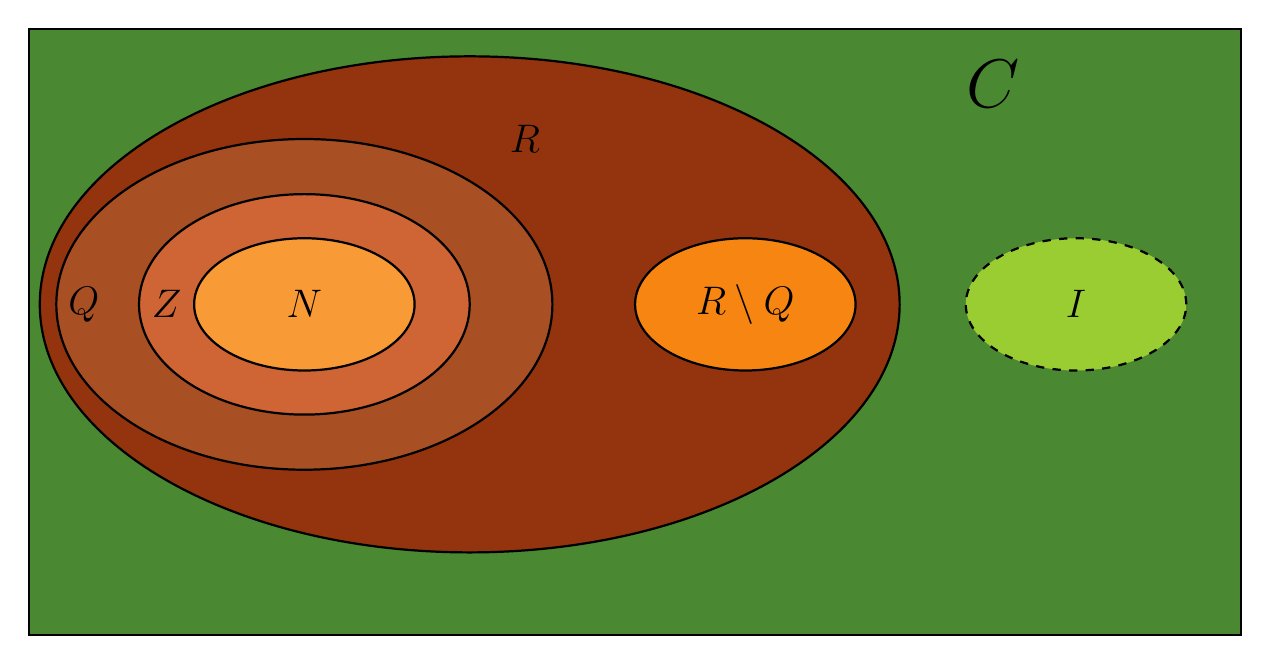
\begin{tikzpicture}[scale=0.7]

    % Complex Numbers (outer square)
    \draw[thick, fill=OliveGreen!90] (-12, -6) rectangle (10, 5);
    \node at (5.5, 4) {\Huge $\mathbb{C}$};
    
    % Real Numbers (largest set)
    \draw[thick, fill=RawSienna] (-4,0) ellipse (7.8cm and 4.5cm);
    \node at (-3, 3) {\Large $\mathbb{R}$};
    
    % Rational Numbers
    \draw[thick, fill=RawSienna!80] (-7,0) ellipse (4.5cm and 3cm);
    \node at (-11, 0) {\Large$\mathbb{Q}$};
    
    % Integers
    \draw[thick, fill=Bittersweet!75] (-7,0) ellipse (3cm and 2cm);
    \node at (-9.5, 0) {\Large$\mathbb{Z}$};
    
    % Natural Numbers
    \draw[thick, fill=BurntOrange!80] (-7,0) ellipse (2cm and 1.2cm);
    \node at (-7, 0) {\Large$\mathbb{N}$};
    
    % Irrational Numbers
    \draw[thick, fill=BurntOrange] (1,0) ellipse (2cm and 1.2cm);
    \node at (1, 0) {\Large$\mathbb{R} \setminus \mathbb{Q} $};
    
    % Imaginary Numbers
    \draw[thick, dashed, fill=YellowGreen] (7,0) ellipse (2cm and 1.2cm);
    \node at (7, 0) {\Large $\mathbb{I}$};

\end{tikzpicture}
    \caption{Venn diagram of numbers}
    \label{fig:venn_num}
\end{figure}

Throughout history, number theory has evolved from a purely theoretical pursuit to a field with practical applications in modern technology. For example, cryptography, the science of securing communication, relies heavily on number theory, particularly the properties of prime numbers and modular arithmetic. The algorithms that protect our online transactions and digital communications are built upon the principles of number theory.

In this chapter, we will explore various aspects of numbers and number theory, starting with the basics of integers, prime numbers, and number systems, and gradually advancing to more complex topics. By understanding the fundamental properties of numbers, we gain insights into the mathematical structures that underpin the digital world and beyond.

\begin{remark}
Many numbers are included in more than one set. Table \ref{tab:number_types} offers an overview of the names, properties of and symbols used for the main number types.
\end{remark}

\begin{table}[ht]
\centering
\caption{Types of Numbers and Their Properties}
\label{tab:number_types}
\renewcommand{\arraystretch}{1.6} % Adjust the row height for the entire table
\begin{tabular}{|m{3.1cm}|>{\centering\arraybackslash}m{1.5cm}|m{5.4cm}|m{5cm}|}
\hline
\raggedright\text{Natural Numbers} & \(\mathbb{N}\) & Numbers used for counting (all positive integers). & \(0, 1, 2, \ldots\) \\ \hline
\raggedright\text{Integers} & \(\mathbb{Z}\) & All positive and negative whole numbers. & \(\{\ldots, -2, -1, 0, 1, 2, \ldots\}\) \\ \hline
\raggedright\text{Rational Numbers} & \(\mathbb{Q}\) & All real numbers which can be expressed as a fraction, \(\frac{p}{q}\), where \(p\) and \(q\) are integers and \(q \neq 0\). All integers are rational numbers as \(1\) is a non-zero integer. & \(\dfrac{1}{5}, \dfrac{5}{1} (=5), \dfrac{2}{3}, \dfrac{3}{2}, \dfrac{0}{3} (=0)\) \\ \hline
\raggedright\text{Irrational Numbers} & \(\mathbb{R}\ \setminus \mathbb{Q}\) & All real numbers which cannot be expressed as a fraction whose numerator and denominator are integers (i.e., all real numbers which aren't rational). & \(\pi, \sqrt{2}, \sqrt{3}\) \\ \hline
\raggedright\text{Real Numbers} & \(\mathbb{R}\) & Includes all numbers on the number line. & \(\dfrac{1}{5}, \sqrt{\dfrac{1}{5}}, 0, -2\) \\ \hline
\raggedright\text{Imaginary Numbers} & \(\mathbb{I}\) & Numbers which are the product of a real number and the imaginary unit \(i\) (where \(i = \sqrt{-1}\)). & \(\begin{array}{l}
\vspace{3pt} 3i = \sqrt{-9},\ -5i = \sqrt{-25}, \\
3\sqrt{2}i = \sqrt{-18} \vspace{3pt}
\end{array}\) \\ \hline
\raggedright\text{Complex Numbers} & \(\mathbb{C}\) & All numbers which can be expressed in the form $a+b i$ where $a$ and $b$ are real numbers and $i=\sqrt{-1}$. Each complex number is a combination of a real number $(a)$ and an imaginary number $(b i)$. & $1+2 i, 1, i,-3 i, 0,-5+i$ \\ \hline
\end{tabular}
\end{table}

\begin{remark}
    Figure \ref{fig:venn_num} may appear misleading at first glance, as it suggests that there are real numbers which are neither rational nor irrational (depicted by the blue region). However, this is not the case. The set of real numbers is exclusively comprised of rational and irrational numbers. This is precisely why the set of irrational numbers is denoted as \(\mathbb{R} \setminus \mathbb{Q}\), meaning "all real numbers except the rational numbers". The same is true of the complex numbers; the are all composed of the real numbers and the imaginary numbers.
\end{remark}

\section{Types of Numbers}
Let's explore the various types of numbers, including natural numbers, whole numbers, integers, rational numbers, irrational numbers, and real numbers - imaginary numbers and complex numbers are left out of this discussion.

\subsection*{Natural Numbers}
We begin with the natural numbers. We distinguish between whole numbers: $0, 1, 2, 3, \ldots$ and counting numbers: $1, 2, 3, \ldots$. These numbers are primarily used for counting. Natural numbers are often regarded as exact values (e.g., there are 4 tires on a car, 8 legs on a spider). However, in some contexts, they may be used as approximations (e.g., there were approximately 1000 people in the crowd).

One of the key properties of natural numbers is that they are \textit{closed} under certain operations, such as addition and multiplication. This means that if you take any two natural numbers and add or multiply them, the result will always be another natural number. For example, if $a$ and $b$ are natural numbers, then both $a + b$ and $a \times b$ are also natural numbers.

There is very little consensus as to whether the symbol $\mathbb{N}$ includes 0. Therefore, the set of whole numbers (that include 0) is often denoted $\mathbb{W}$.

\subsection*{Integers}
Integers are the basic building blocks of number theory, consisting of the set of whole numbers and their negatives. Formally, integers include numbers like $\ldots,-3,-2,-1,0,1,2,3, \ldots$ Basic arithmetic operations, such as addition and multiplication, follow certain properties:

\begin{custombox}{{Commutative, Associative, and Distributive Laws}}


    \begin{itemize}
    \item Commutativity: $a+b=b+a$
    \item Associativity: $(a+b)+c=a+(b+c)$
    \item Distributive property: $a \times(b+c)=a \times b+a \times c$
    \end{itemize}
    
\end{custombox}

Integers are a fundamental set of numbers in mathematics, denoted by the symbol $\mathbb{Z}$. This set includes all the positive and negative whole numbers, as well as zero. Integers extend the natural numbers by incorporating their additive inverses, thereby allowing for the complete operation of subtraction within the set.

\textbf{Additive Identity:} The number \(0\) is known as the additive identity. This is because for any integer \(a\), adding zero does not change the value of \(a\). In mathematical terms, this property is expressed as \(0 + a = a + 0 = a\). This identity is crucial because it ensures that the set of integers remains stable under addition.
    
 \textbf{Multiplicative Identity:} Similarly, the number \(1\) serves as the multiplicative identity. For any integer \(a\), multiplying by one leaves the value of \(a\) unchanged: \(1 \times a = a \times 1 = a\). This property underpins the stability of integers under multiplication, maintaining the integrity of the set.
    
\textbf{Additive Inverse:} For each integer \(a\), there exists a corresponding additive inverse, denoted as \(-a\). The additive inverse is defined such that when \(a\) and \(-a\) are added together, the result is the additive identity, zero: \(a + (-a) = 0\). This property allows for the operation of subtraction within the set of integers, as subtraction can be viewed as the addition of an additive inverse.

\begin{custombox}{Closure Property}
    \textbf{Addition:} The set of integers is closed under the operation of addition. This means that if you take any two integers and add them together, the sum will always be an integer. For example, if \(a\) and \(b\) are integers, then \(a + b\) is also an integer. This closure property ensures that the set of integers is stable and complete under addition, meaning that no matter how many times you add integers together, the result will remain within the set of integers.

\textbf{Multiplication:} The set of integers is also closed under multiplication. If you multiply any two integers, the product will always be an integer. For instance, if \(a\) and \(b\) are integers, then \(a \times b\) is also an integer. This property guarantees that the operation of multiplication, like addition, does not produce results outside the set of integers, thereby preserving the integrity of the set under multiplication.

\end{custombox}

It is universally agreed upon that the definition of an integer is clear and precise. Therefore, when in doubt, it is advisable to refer to numbers within this set as "integers." When you specifically need to refer to only the positive integers, it is both accurate and professional to explicitly state "positive integers." This terminology not only ensures clarity but also reflects a sound understanding of mathematical conventions. 

Remember, zero is neither positive nor negative, so when discussing subsets of integers, careful consideration of this fact is necessary:

\begin{itemize}
    \item \textbf{Integers:} $\mathbb{Z} = \{\ldots,-4,-3,-2,-1,0,1,2,3,4, \ldots\}$
    \item \textbf{Negative Integers:} $\mathbb{Z}^- = \{\ldots,-4,-3,-2,-1\}$
    \item \textbf{Positive Integers:} $\mathbb{Z}^+ = \{1,2,3,4, \ldots\}$
    \item \textbf{Non-Negative Integers:} $\mathbb{Z}_0^+ = \mathbb{Z}_{\geq 0} = \{0,1,2,3,4, \ldots\}$
    \item \textbf{Non-Positive Integers:} $\mathbb{Z}_0^- = \mathbb{Z}_{\leq 0} = \{\ldots,-4,-3,-2,-1, 0\}$
\end{itemize}

This notation should be consistent with standard mathematical conventions.

\subsection*{Rational Numbers}
Rational numbers, denoted by the symbol $\mathbb{Q}$, are numbers that can be expressed as the quotient of two integers, where the numerator is any integer and the denominator is a non-zero integer. Formally, a rational number can be written as $\frac{a}{b}$, where $a \in \mathbb{Z}$ and $b \in \mathbb{Z} \setminus \{0\}$. This set of numbers is fundamental in mathematics as it provides a means to represent fractions and ratios, allowing for a wide range of arithmetic operations, and as such are a generalisation of common fractions which we saw in \autoref{chap:ch1}. They can represent any number that can be written as a finite or repeating decimal.

One of the key properties of rational numbers is that each non-zero rational number has a \textit{multiplicative inverse}. The multiplicative inverse of a rational number $\frac{a}{b}$ is the rational number $\frac{b}{a}$, provided that $a \neq 0$. The importance of the multiplicative inverse lies in the fact that when a number is multiplied by its inverse, the result is the \textit{multiplicative identity}, which is 1. In other words, for any rational number $\frac{a}{b}$, its inverse is denoted by $\left(\frac{a}{b}\right)^{-1} = \frac{b}{a}$, and we have:

\[
\frac{a}{b} \times \frac{b}{a} = \frac{ab}{ba} = 1
\]

This property ensures that rational numbers are closed under multiplication and division (except division by zero), making them a robust and versatile set of numbers for various mathematical operations.

Rational numbers are dense on the number line, meaning that between any two rational numbers, there exists another rational number. This property makes the set of rational numbers particularly important in the study of real numbers, as it allows for the approximation of irrational numbers to any desired degree of accuracy.

\subsection*{Irrational Numbers}
Irrational numbers, denoted by the symbol $\mathbb{R} \setminus \mathbb{Q}$, are real numbers that cannot be expressed as the quotient of two integers. Unlike rational numbers, which have a repeating or terminating decimal expansion, the decimal expansion of an irrational number neither repeats nor terminates. This property makes irrational numbers fundamentally different from rational numbers, as they cannot be precisely represented as fractions.

Some of the most famous examples of irrational numbers include:

\begin{itemize}
    \item \textbf{Pi} ($\pi$): Perhaps the most well-known irrational number, $\pi$ is the ratio of the circumference of a circle to its diameter. Its value is approximately $3.14159\ldots$, but its decimal expansion goes on infinitely without repeating. $\pi$ plays a crucial role in geometry, trigonometry, and calculus.

    \item \textbf{The Golden Ratio} ($\phi$): The golden ratio, $\phi \approx 1.61803\ldots$, is an irrational number that appears frequently in nature, art, and architecture. It is defined as the positive solution to the equation $x^2 - x - 1 = 0$, and it is the limit of the ratio of successive Fibonacci numbers.

    \item \textbf{The Square Root of 2} ($\sqrt{2}$): The square root of 2, approximately $1.41421\ldots$, is the length of the diagonal of a square with side length 1. This number is historically significant because its discovery by the ancient Greeks, particularly the Pythagoreans, revealed the existence of numbers that could not be expressed as the ratio of two integers. The Pythagorean theorem states that in a right triangle, the square of the hypotenuse is equal to the sum of the squares of the other two sides. For a right triangle with both legs of length 1, the hypotenuse is $\sqrt{2}$, demonstrating that $\sqrt{2}$ cannot be a rational number.

    \item \textbf{Euler's Number} ($e$): The number $e \approx 2.71828\ldots$ is the base of the natural logarithm and is a fundamental constant in mathematics, particularly in calculus and complex analysis. The number $e$ arises naturally in various growth processes, such as compound interest and population growth.
\end{itemize}

Irrational numbers fill the gaps between rational numbers on the number line, making the real numbers a continuous set. However, like rational numbers, they too have important properties. For instance, while irrational numbers do not have a simple fractional representation, they are nonetheless essential in representing the lengths, areas, and volumes that cannot be captured by rational numbers alone.

\subsection*{Real Numbers}
Real numbers, denoted by the symbol $\mathbb{R}$, form the foundation of most mathematical analysis and are essential in describing continuous quantities. The set of real numbers is composed of both rational numbers ($\mathbb{Q}$) and irrational numbers ($\mathbb{R} \setminus \mathbb{Q}$), thus encompassing all numbers that can be placed on the number line. While both rational and irrational numbers are part of the real number system, they differ significantly in their properties:

\begin{custombox}{Similarities and Differences of Rational and Irrational Numbers}
    \begin{itemize}
    \item \textbf{Representation:} Rational numbers can be represented as fractions, while irrational numbers cannot. This distinction makes irrational numbers more complex to handle, especially in arithmetic operations.

    \item \textbf{Decimal Expansion:} The decimal expansion of rational numbers is either finite or periodic, while that of irrational numbers is infinite and non-repeating.

    \item \textbf{Closure Properties:} Rational numbers are closed under addition, subtraction, multiplication, and division (except by zero). Irrational numbers are not closed under these operations; for example, the sum or product of two irrational numbers can sometimes be rational.

    \item \textbf{Density:} Rational numbers are dense on the real number line, meaning that between any two rational numbers, there exists another rational number. Irrational numbers are also densely distributed but in a complementary manner, filling in the "gaps" left by the rationals, ensuring that the real number line is continuous without any breaks.
\end{itemize}
\end{custombox}

The real number line is a continuous, unbroken line that extends infinitely in both directions. Every point on this line corresponds to a unique real number, whether rational or irrational. This continuity is what allows the real numbers to model continuous phenomena in nature, such as time, distance, and temperature.

\section{Integer Properties and Modular Arithmetic}
In \ref{chap:ch1} we introduced the concept of a factor. A factor is a portion of a quantity, usually an integer or polynomial that, when multiplied by other factors, gives the entire quantity.

In number theory, a factor of a number \(n\) is synonymous with a \textbf{divisor} of \(n\). Specifically, a divisor of an integer \(n\) is an integer \(d\) that divides \(n\) and results in another integer.

A positive \textbf{proper divisor} is a positive divisor of a number \(n\), excluding \(n\) itself. Similarly, a \textbf{proper factor} of a positive integer \(n\) is a factor of \(n\) other than 1 or \(n\).

For example, the factors of 12 are:

\[
1, 2, 3, 4, 6, 12
\]

In this list, 2, 3, 4, and 6 are proper factors of 12, meaning they are less than 12 itself but greater than 1.

A prime number is a natural number greater than 1 that has no positive divisors other than 1 and itself. In other words, a prime number cannot be formed by multiplying two smaller natural numbers. The first few prime numbers are:

\[
2, 3, 5, 7, 11, 13, 17, 19, 23, 29, \ldots
\]

Notice that 2 is the only even prime number because any other even number can be divided by 2, making it \textit{composite}. A \textbf{composite number}, in contrast to a prime, is a natural number greater than 1 that can be divided evenly by at least one positive integer other than 1 and itself. For example, 6 is a composite number because it can be expressed as \(6 = 2 \times 3\).

\subsection*{Prime factorisation}
Prime factorisation is the process of breaking down a composite number into a product of its prime factors. For any composite number, this factorisation is unique, except for the order of the factors. For instance, consider the number 60:
\[
60 = 2 \times 2 \times 3 \times 5 = 2^2 \times 3 \times 5
\]
Here, 2, 3, and 5 are prime factors of 60 and $2^2 \times 3 \times 5$ is the \textbf{canonical factorisation} of 60 - we usually just call it the prime factorisation.

\begin{theorem}{The Fundamental Theorem of Arithmetic}
Every integer greater than 1 can be represented uniquely as a product of prime numbers, up to the order of the factors.
\end{theorem}

This theorem underscores the importance of prime numbers as the "building blocks" of all natural numbers.

\begin{example}

\[
84 = 2^2 \times 3 \times 7
\]
\end{example}

No matter how you factorise 84, you will always end up with this set of prime numbers (2, 3, and 7), though the order might differ.

The prime factorisation allows for a unique representation of the number in terms of its prime factors.

\subsection*{Greatest Common Divisor (GCD)}
The Greatest Common Divisor (GCD), also referred to as the \textit{highest common factor} (HCF) or \textit{greatest common factor} (GFC), of two or more integers is the largest positive integer that divides each of the given integers without leaving a remainder. To determine the GCD, one commonly employs the prime factorisation of the numbers involved. The GCD is then found by multiplying the common prime factors with the smallest exponents from the prime factorisation of the numbers.

For example, consider finding the GCD of 24 and 36:
\[
24 = 2^3 \times 3, \quad 36 = 2^2 \times 3^2
\]
The common prime factors are 2 and 3. Thus, the GCD is:
\[
\text{GCD} = 2^2 \times 3 = 12
\]

\begin{example} Find the GCD of 36 and 120

\begin{solution}
    

The arrows indicate the numbers that we chose.

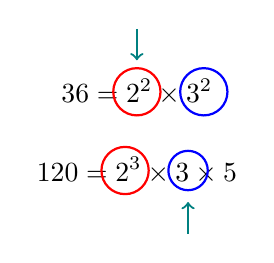
\begin{tikzpicture}
    % First line
    \node at (0, 0) {\(\displaystyle 36 = 2^2 \times 3^2\)};
    
    % Second line
    \node at (0, -1) {\(\displaystyle 120 = 2^3 \times 3 \times 5\)};
    
    % Circles around specific elements
    \draw[red, thick] (0, 0.0) circle(0.3); % Circle around 2^2
    \draw[blue, thick] (0.85, 0.0) circle(0.3); % Circle around 3^2
    
    \draw[red, thick] (-0.15, -1) circle(0.3); % Circle around 2^3
    \draw[blue, thick] (0.65, -1) circle(0.25); % Circle around 3

    % Arrows
    \draw[thick, teal, ->] (0, 0.8) -- (0, 0.4);
    \draw[thick, teal, ->] (0.65, -1.8) -- (0.65, -1.4);
\end{tikzpicture}

We see that 2 and 3 are common factors, and choose the ones with the smallest exponents:

\[
GCD = 2^2\times 3 = 12
\]
\end{solution}

\end{example}
 
\subsection*{Least Common Multiple (LCM)}
The Least Common Multiple (LCM) of two or more integers is the smallest positive integer that is evenly divisible by each of the given integers. The LCM can also be determined using the prime factorisation of the numbers. 

For instance, to find the LCM of 24 and 36:
\[
24 = 2^3 \times 3, \quad 36 = 2^2 \times 3^2
\]
The LCM is obtained by taking the highest power of each prime factor that appears in the factorisation of either number:
\[
\text{LCM} = 2^3 \times 3^2 = 72
\]

\begin{example} Find the LCM of 12 and 18

\begin{solution}
\[
15 = 3\times 5
\]
\[
18 = 2 \times 3^2
\]

So the factors with the highest exponents in either factorisation is $2$, $3^2$, and $5$, so

\[
LCM = 2 \times 3^2 \times 5 = 90
\]
    
\end{solution}
    
\end{example}

\begin{example} Find the LCM of 80 and 120

\begin{solution}
    

The arrows indicate the numbers that we chose.

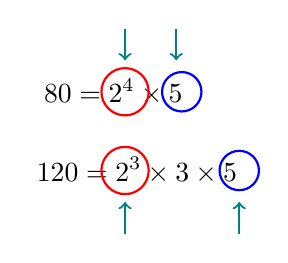
\begin{tikzpicture}
    % First line
    \node at (0, 0) {\(\displaystyle 80 = 2^4 \times 5\)};
    
    % Second line
    \node at (0.3, -1) {\(\displaystyle 120 = 2^3 \times 3 \times 5\)};
    
    % Circles around specific elements
    \draw[red, thick] (0.15, 0.0) circle(0.3); % Circle around 2^2
    \draw[blue, thick] (0.87, 0.0) circle(0.25); % Circle around 3^2
    
    \draw[red, thick] (0.15, -1) circle(0.3); % Circle around 2^3
    \draw[blue, thick] (1.6, -1) circle(0.25); % Circle around 3

    % Arrows
    \draw[thick, teal, ->] (0.15, 0.8) -- (0.15, 0.4);
    \draw[thick, teal, ->] (0.8, 0.8) -- (0.8, 0.4);
    \draw[thick, teal, ->] (0.15, -1.8) -- (0.15, -1.4);
    \draw[thick, teal, ->] (1.6, -1.8) -- (1.6, -1.4);
\end{tikzpicture}

We see that 2 and 5 are common factors and choose the ones with the smallest exponents (5 has the same exponents so we just take one of them):

\[
LCM = 2^4\times 3 \times 5 = 240
\]
\end{solution}

\end{example}


\subsection*{Connection Between GCD and LCM}

An important relationship between the GCD and LCM of two numbers \(a\) and \(b\) is given by the formula:
\[
\text{GCD}(a, b) \times \text{LCM}(a, b) = a \times b
\]
For example, using the numbers 24 and 36:
\[
12 \times 72 = 24 \times 36 = 864
\]
This relationship is a powerful tool in solving problems related to divisibility, number theory, and algebra.

The study of primes and factors is foundational in mathematics, providing essential tools for understanding the structure of numbers. The concepts of prime factorisation, the Fundamental Theorem of Arithmetic, and the calculations of GCD and LCM are not only critical in theoretical mathematics but also in practical applications, such as cryptography, coding theory, and the analysis of algorithms.

\subsection*{Divisors and Remainders}
\label{sec:2.3Mod}
Division involving integers can be tricky since the result might not always be an integer. Often, division produces a remainder. For example,

\[
9 = 2 \times 4 + 1.
\]

In this case, dividing 9 by 4 leaves a \textit{remainder} of 1.

In general, for any integers \(a\) and \(b\), we can express this as:

\[
b = k \times a + r,
\]

where \(r\) is the remainder. If \(r\) is zero, then we say that \(a\) divides \(b\), denoted as \(a \mid b\). The vertical bar is used to signify divisibility. For instance, \(2 \mid 128\) and \(7 \mid 49\), but 3 does not divide 4, which is written as \(3 \nmid 4\).

Above, we made no distinction between factors and divisors. Some argue that they differ slightly:
\begin{itemize}
    \item If $a \mid b$ and $a>0$, $a$ is a \textit{divisor} of $b$.
    \item If $a \notin \{1, b\}$ and $a \mid b$, $a$ is a factor of $b$.
\end{itemize}
In this definition, primes have no factors, only two divisors 1 and itself. We will make no further distinction between primes and factors and use the terms interchangeably.

\subsection*{Modular Arithmetic}
The \texttt{mod} operator, commonly encountered in computer programming, provides the remainder after division. For example:
\begin{enumerate}
    \item \(25 \bmod 4 = 1\) because \(25 \div 4 = 6\) with a remainder of 1.
    \item \(19 \bmod 5 = 4\) since \(19 = 3 \times 5 + 4\).
    \item \(24 \bmod 5 = 4\).
    \item \(99 \bmod 11 = 0\).
\end{enumerate}

While there are some complexities when dealing with negative numbers, we will focus on positive integers for simplicity. It’s also worth noting that the results of the modulus operation are often expressed differently. For instance, \(24 = 4 \bmod 5\) or \(21 = 0 \bmod 7\), which means \(24 \bmod 5 = 4\) and \(21 \bmod 7 = 0\).

Modular arithmetic is sometimes referred to as clock arithmetic. Imagine using a 24-hour clock: 09:00 represents 9 in the morning, while 21:00 represents 9 in the evening. If a journey starts at 07:00 and lasts 25 hours, the arrival time would be 08:00 the next day. Mathematically, this can be expressed as \(7 + 25 = 32\) and \(32 \bmod 24 = 8\). Essentially, we start at 7 and move 25 hours forward on the clock face, landing at 8.
